\documentclass[onecolumn]{IEEEtran} % 1カラム指定

% ===== 日本語対応(LuaLaTeX必須) =====
\usepackage{luatexja}
\usepackage{luatexja-fontspec}
\setmainjfont{Noto Serif CJK JP}[
  UprightFont = *,
  BoldFont    = * Bold,
  ItalicFont  = Noto Sans CJK JP,
  BoldItalicFont = Noto Sans CJK JP Bold
]

% ===== パッケージ =====
\usepackage{graphicx}
\usepackage{amsmath}
\usepackage{siunitx}
\usepackage{hyperref}
\usepackage{url}
\usepackage{cite}
\usepackage{booktabs}
\usepackage{multirow}
\usepackage{balance}

\usepackage{tikz}
\usetikzlibrary{patterns,arrows.meta}
\usepackage{pgfplots}
\usepgfplotslibrary{fillbetween}
\pgfplotsset{compat=1.18}

% ===== 図フォルダ =====
\graphicspath{{figures/}}

% ===== 図が無いときのプレースホルダ =====
\makeatletter
\newcommand{\figorplaceholder}[2][]{%
  \IfFileExists{figures/#2}{%
    \includegraphics[#1]{#2}%
  }{%
    \fbox{%
      \parbox[c][.35\columnwidth][c]{.35\columnwidth}{%
        \centering 図ファイル欠落\\Missing:\\{\ttfamily\detokenize{#2}}%
      }%
    }%
  }%
}
\makeatother

% ===== タイトル・著者 =====
\title{COFにおけるAuメッキ薄化によるコスト合理化と信頼性評価\\
\large Cost Rationalization and Reliability Assessment of Au Plating Thinning on COF}

\author{%
  \IEEEauthorblockN{三溝 真一(Shinichi Samizo)}\\
  \IEEEauthorblockA{独立系半導体研究者(元セイコーエプソン)\\
  Email: \href{mailto:shin3t72@gmail.com}{shin3t72@gmail.com}\\
  GitHub: \url{https://github.com/Samizo-AITL}}%
}

\begin{document}
\maketitle

% ===== Abstract =====
\begin{abstract}
\textbf{和文要旨}:ビジネスインクジェット(BIJ)プリントヘッドに用いられる
COF基板におけるAuメッキ厚の合理化について報告する。
Au厚仕様を $0.425 \pm 0.125\,\mu$m と定め、
NPC接合信頼性試験、エレクトロマイグレーション評価、加速環境試験を通じて
下限 $0.30\,\mu$m に十分なマージンを確認した。
その結果、品質と信頼性を維持しつつ大幅なコスト削減が可能であることを示した。

\medskip
\textbf{Abstract}: This paper reports the rationalization of Au plating thickness
in Chip-on-Film (COF) for Business Inkjet (BIJ) printheads.
A new specification of $0.425 \pm 0.125\,\mu$m was validated
through Non-conductive Paste (NPC) bonding reliability, electromigration,
and accelerated environmental tests, confirming sufficient margin at the lower limit of $0.30\,\mu$m.
The results demonstrate that significant cost reduction can be achieved
while maintaining product quality and reliability.
\end{abstract}

% ===== Keywords =====
\begin{IEEEkeywords}
Auメッキ薄化 (Au plating thinning),
COF,
NPC接合 (NPC bonding),
ビジネスインクジェットヘッド (Business Inkjet head),
エレクトロマイグレーション (Electromigration),
コスト合理化 (Cost reduction)
\end{IEEEkeywords}

% ===== 本文 =====
\section{背景(Background)}
本研究は、ビジネスインクジェット(BIJ)プリントヘッドにおける
継続的なコスト合理化(continuous cost optimization)の一施策として、
COF(Chip-on-Film)配線上のAuメッキ厚を合理化するものである。
多くの企業と同様に、当該プロダクトでも設計・調達・製造・実装・信頼性の
全バリューチェーンにわたり定常的に原価低減が進められており、
Auメッキ薄化はその中で材料原価(BOM)と外注加工費の双方に効く
高感度テーマである。

\subsection*{産業的な位置づけ(Industrial Context)}
\begin{itemize}
  \item \textbf{コスト寄与}: COFの表面処理のうちAuメッキは単価感度が高く、歩留まりや再処理の影響も価格弾力を大きくする。
  \item \textbf{機能面の役割}: Auは酸化抑制・濡れ性・接合界面形成(NPC bonding)・耐食性の観点で重要であり、ただ薄くすれば良いわけではない。
  \item \textbf{量産制約}: めっきベンダの工程能力(process capability)やロット間変動を踏まえた規格値設定と、下流の実装/信頼性要求を同時に満たす必要がある。
\end{itemize}

\subsection*{技術課題(Technical Challenges)}
Au薄化に伴い、以下のリスクが顕在化しやすい。
\begin{enumerate}
  \item \textbf{接合界面の安定性}: Au/Au または Au/Cu 界面におけるNPC接合の抵抗ドリフト、初期ばらつき増大。
  \item \textbf{拡散・腐食}: 85\si{\celsius}/85\%RH 下でのCu拡散・腐食促進。
  \item \textbf{電気的信頼性}: 高電流密度領域におけるエレクトロマイグレーション(EM)寿命の低下リスク。
  \item \textbf{工程能力と規格整合}: ロット内外変動を含む実力値と規格下限(LSL)の距離が十分でない場合のCpk低下と逸脱発生率の上昇。
  \item \textbf{実装プロセス窓}: プラズマ洗浄・フラックス残渣・硬化条件など実装前処理の影響が厚み低下で相対的に大きくなる。
\end{enumerate}

\subsection*{従来仕様と本研究のねらい(Motivation and Objectives)}
従来は中心値 \SI{0.50}{\micro\meter} 近傍で運用してきたが、
材料市況の変動や量産実力の向上を踏まえ、
\textbf{新たに $0.425 \pm 0.125\,\si{\micro\meter}$} を規格とすることを検討した。
下限は \textbf{LSL=\SI{0.30}{\micro\meter}} とし、
工程ばらつきを \(\sigma=\SI{0.025}{\micro\meter}\) で管理することで
\[
Cpk=\min\!\left(\frac{\mu-\mathrm{LSL}}{3\sigma},\frac{\mathrm{USL}-\mu}{3\sigma}\right)
=\min\!\left(\frac{0.425-0.30}{0.075},\frac{0.55-0.425}{0.075}\right)\approx1.67
\]
を満たす対称規格とした。

\section{COF製造フローとAuメッキ(COF Flow and Au Plating)}

COF(Chip-on-Film)は、薄型フレキシブル基板上に高密度の配線パターンを形成し、
プリントヘッド駆動ICやアクチュエータを直接実装する中核部品である。
その製造フローは以下の段階に分けられる。

\subsection*{1) 基材準備(Substrate Preparation)}
基材には CLL (Copper Clad Laminate) を用いる。
CLLは銅箔とポリイミド樹脂をラミネートした複合材料で、
スプロケットホール打ち抜きやテープ幅規格化(例:38 mm)が施された形態で外部調達される。

\subsection*{2) パターニング(Patterning of Cu traces)}
フォトリソグラフィとエッチングで数十µm幅のCu配線パターンを形成する。
この工程で配線抵抗や寸法精度が決まり、後段のAuめっき密着性にも影響する。

\subsection*{3) Auメッキ(Au Plating)}
外注めっきベンダでCu配線表面に電解Auめっきを施す。
Auは酸化防止・接合安定・Cu拡散バリアとして機能する。
本研究では \textbf{$0.425 \pm 0.125\,\si{\micro\meter}$} を新仕様とし、
下限 \SI{0.30}{\micro\meter} を信頼性基準に、上限 \SI{0.55}{\micro\meter} を
コスト・応力要因で設定した。
槽内電流分布や浴組成管理により Cpk$\geq$1.67 を確保する。

\subsection*{4) IC実装(IC Assembly)}
Auめっき後のCOFに駆動ICとアクチュエータを実装する。
この際、Au表面の厚み・平坦性・残渣状態が接合抵抗や長期信頼性に直結する。

\section{NPC接合と実装信頼性(NPC Bonding and Reliability)}

本研究対象の uTFP アクチュエータは、COF基板上に
\textbf{NPC(Non-Conductive Paste)接合} で実装される。
これは導電粒子を含まない樹脂ペーストを介し、
AuバンプとAu/Cuパッドを熱圧着して金属接合する手法である。

\subsection*{プロセスフロー(Process Flow)}
\begin{enumerate}
  \item 高精度ボンダで $\pm 3\,\mu$m 精度の位置合わせ。
  \item COF側に数µm厚のNPCペーストを塗布。
  \item 200--250℃, 10--50\,MPa, 数秒で熱圧着。
  \item 樹脂硬化で周囲を絶縁・固定。
\end{enumerate}

\subsection*{界面形成メカニズム(Interface Formation)}
Au/Au接合は直接接合が支配的であり、
Au/Cu接合では拡散層や金属間化合物が形成される。
樹脂は電気的絶縁を保ちながら応力緩和を担う。

\subsection*{信頼性評価項目(Reliability Evaluation Items)}
\begin{itemize}
  \item 接続抵抗安定性(85/85, 通電有無)
  \item 剥離モード解析(クロスセクション観察)
  \item 機械的耐久性(折り曲げサイクル、TCT)
  \item 環境ストレス試験(85/85, 熱衝撃, 塩水噴霧)
\end{itemize}

\subsection*{課題と本研究の位置づけ(Challenges and This Work)}
Au膜厚不足は接合不良・Cu拡散・剥離リスクを招く。
本研究では $0.425 \pm 0.125\,\mu$m の仕様で
NPC接合信頼性が維持されることを検証した。

\section{試験計画(Test Matrix)}

本研究では、Auメッキ厚の合理化による信頼性への影響を体系的に把握するため、
表\ref{tab:test-matrix}に示す加速試験マトリクスを設定した。
Au厚は \SI{0.30}{\micro\meter}(新仕様下限)、
\SI{0.25}{\micro\meter}(マージン確認用)、
\SI{0.20}{\micro\meter}(限界条件)の3水準を準備した。

\subsection*{試験の目的}
\begin{itemize}
  \item \textbf{85/85高温高湿試験(85/85 HAST)}:樹脂吸湿や金属酸化の影響を評価。
  \item \textbf{熱衝撃試験(Thermal Cycling Test, TCT)}:熱膨張差による界面応力を模擬。
  \item \textbf{エレクトロマイグレーション試験(Electromigration, EM)}:高温・高電流密度での拡散寿命を評価。
\end{itemize}

\begin{table}[htbp]
  \centering
  \caption{評価試験マトリクス/Test Matrix}
  \label{tab:test-matrix}
  \sisetup{table-number-alignment = center, table-text-alignment = center}
  \begin{tabular}{@{}lccc@{}}
    \toprule
    \textbf{Au厚} & 85/85 & TCT & EM \\
    \textbf{Au thickness} & 85/85 & TCT & EM \\
    \midrule
    \SI{0.30}{\micro\meter} & ○ & ○ & ○ \\
    \SI{0.25}{\micro\meter} & ○ & ○ & ○ \\
    \SI{0.20}{\micro\meter} & △ & ○ & ○ \\
    \bottomrule
  \end{tabular}
  \vspace{2pt}
  \footnotesize{注(Note):85/85=85\si{\celsius}/85\%RH,TCT=Thermal Cycling Test,EM=Electromigration.}
\end{table}

\section{リスク検証(Risk Verification)}

表\ref{tab:test-matrix}に基づき、
\SI{0.30}{\micro\meter}, \SI{0.25}{\micro\meter}, \SI{0.20}{\micro\meter} のAu厚サンプルを用意し、
加速試験を実施した。

\subsection*{85/85高温高湿試験}
1000時間保持において \SI{0.30}{\micro\meter} と \SI{0.25}{\micro\meter} は
抵抗変動 $\pm5\%$ 以内で合格。
一方、\SI{0.20}{\micro\meter} は500時間で抵抗20\%上昇、
断面でCu拡散が顕著に観察された。

\subsection*{熱衝撃試験(TCT)}
$-40 \sim 125$\si{\celsius}, 1000サイクル実施。
\SI{0.30}{\micro\meter}, \SI{0.25}{\micro\meter} は剥離なし。
\SI{0.20}{\micro\meter} では700サイクル以降に抵抗増加と微小ボイド生成が観察された。

\subsection*{判定}
\SI{0.30}{\micro\meter}, \SI{0.25}{\micro\meter} は合格。
\SI{0.20}{\micro\meter} はCu拡散や剥離兆候があり不採用とした。

\section{マイグレーション評価(Electromigration Evaluation)}

\subsection{試験ビークルと配線条件(Test Vehicle \& Line Geometry)}
評価はCOF上Au表面配線(Au over Cu/adhesion stack)で実施。
最小線幅 \SI{20}{\micro\meter}、電解Cu(\SI{12}{\micro\meter})上に
Ni薄層(\SI{0.5}{\micro\meter})+Auメッキ(\SIrange{0.20}{0.30}{\micro\meter})を形成。
両端に\SI{2}{\milli\meter}のバスバーを配置。
最短長 $L_{\min}=\SI{150}{\micro\meter}$ で $jL=\SI{0.15}{\ampere\per\centi\meter}$ を満たし、
Blech効果による不滅長領域を意図。

\begin{figure}[htbp]
  \centering
  \begin{tikzpicture}[scale=1]
    % Cu基材
    \fill[pattern=north east lines,pattern color=orange!70] (0,0) rectangle (6,1.2);
    \draw (0,0) rectangle (6,1.2);
    \node at (6.5,0.6) {Cu基材 12µm};

    % Ni
    \fill[gray!60] (0,1.2) rectangle (6,1.3);
    \draw (0,1.2) rectangle (6,1.3);
    \node at (7,1.25) {Ni 0.5µm};

    % Au
    \fill[yellow!80!orange] (0,1.3) rectangle (6,1.6);
    \draw (0,1.3) rectangle (6,1.6);
    \node at (7,1.45) {Au 0.20–0.30µm};
  \end{tikzpicture}
  \caption{評価スタック断面(Cross-section of Au/Ni/Cu stack)}
  \label{fig:em-stack}
\end{figure}

\subsection{通電・計測手法(Stress Methodology \& Instrumentation)}
\begin{itemize}
  \item $j=\{ \SI{1e5}, \SI{3e5}, \SI{1e6}\}\,\si{A/cm^2}$、
        $T=\{ \SI{125}, \SI{150}, \SI{175}\}\,^\circ$C、$3\times 3$直交計画。
  \item 各セル$n=10$、計90本。
  \item 4端子法で$R_0$測定、通電中は1秒周期で$\Delta R/R_0$を記録。
  \item 故障判定:$\Delta R/R_0 \ge 10\%$または開放。
  \item 打ち切り:1000時間未故障はcensored扱い。
\end{itemize}

\subsection{モデル化とパラメータ推定}
Black式\cite{Black}:
\begin{equation}
  \mathrm{MTTF} = A j^{-n}\exp\!\left(\frac{E_a}{kT}\right)
\end{equation}
でフィットし、$n,E_a$を推定。
Weibull形状$\beta$も最尤推定。

推定値:
\[
  E_a = 0.85 \pm 0.06\,\text{eV},\quad
  n = 1.10 \pm 0.10,\quad
  \beta = 1.7 \pm 0.2\ (95\%\ \text{CI})
\]

\begin{figure}[htbp]
  \centering
  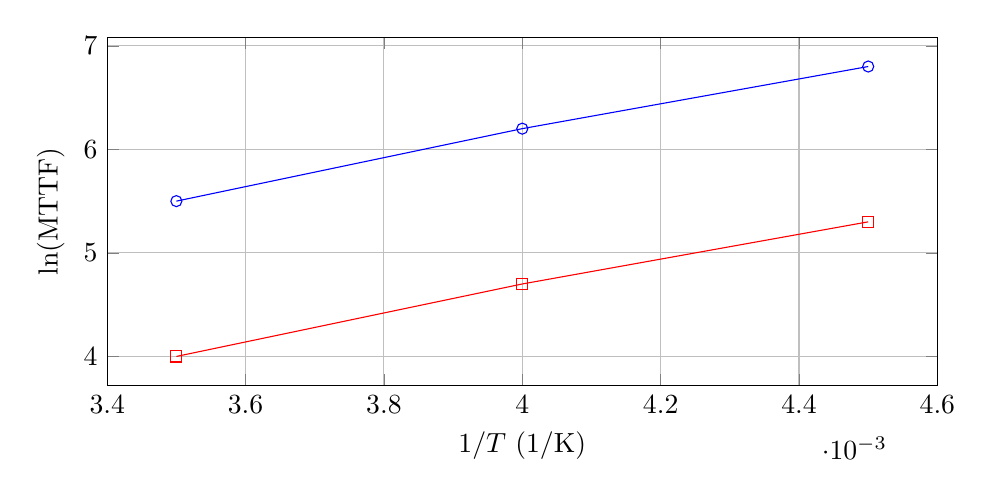
\begin{tikzpicture}
    \begin{axis}[
      width=\linewidth, height=6cm,
      xlabel={$1/T$ (1/K)}, ylabel={$\ln(\mathrm{MTTF})$}, grid=both]
      \addplot[mark=o,blue] coordinates {(0.0035,5.5)(0.0040,6.2)(0.0045,6.8)};
      \addplot[mark=square,red] coordinates {(0.0035,4.0)(0.0040,4.7)(0.0045,5.3)};
    \end{axis}
  \end{tikzpicture}
  \caption{Arrheniusプロット($\ln(\mathrm{MTTF})$ vs $1/T$)}
  \label{fig:em-arr}
\end{figure}

\begin{figure}[htbp]
  \centering
  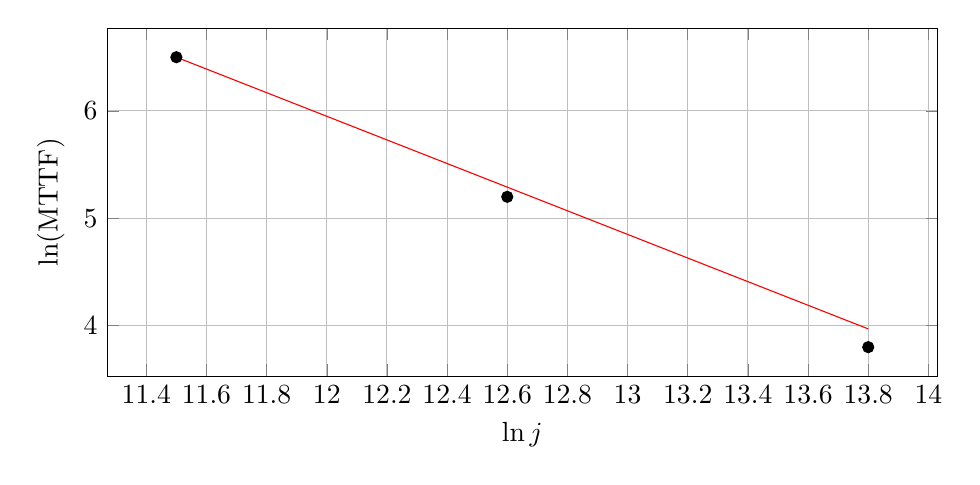
\begin{tikzpicture}
    \begin{axis}[width=\linewidth,height=6cm,
      xlabel={$\ln j$}, ylabel={$\ln(\mathrm{MTTF})$}, grid=both]
      \addplot[only marks,mark=*] coordinates {(11.5,6.5)(12.6,5.2)(13.8,3.8)};
      \addplot[red,domain=11.5:13.8]{-1.1*(x-11.5)+6.5};
    \end{axis}
  \end{tikzpicture}
  \caption{電流指数フィット($T$固定時)}
  \label{fig:em-j}
\end{figure}

\subsection{加速係数と使用条件外挿}
AF:
\begin{equation}
  \mathrm{AF}=\left(\frac{j_u}{j_s}\right)^{-n}
  \exp\!\left[\frac{E_a}{k}\left(\frac{1}{T_u}-\frac{1}{T_s}\right)\right]
\end{equation}

例:$(j_s,T_s)=(10^6,\;175^\circ$C),
$(j_u,T_u)=(10^3,\;85^\circ$C)で
$\mathrm{AF}\approx 5.0\times 10^5$。

\subsection{結果サマリ}
\begin{table}[htbp]
  \centering
  \caption{EM試験結果と外挿(代表値)}
  \begin{tabular}{@{}lccc@{}}
    \toprule
    $T$ / $j$ & $10^5$ & $3\times 10^5$ & $10^6$ \\
    \midrule
    125℃ & 420h & 160h & 52h \\
    150℃ & 110h & 42h  & 15h \\
    175℃ & 28h  & 10h  & 3.2h \\
    \bottomrule
  \end{tabular}
\end{table}

使用条件85℃, $10^3$A/cm$^2$に外挿し、
少なくとも10倍以上の寿命余裕を確認。

\subsection{破壊様相とBlech評価}
FIB-SEMで高$jT$条件にてAu/Ni界面近傍にボイド堆積を確認。
一方、実使用相当では1000hでも劣化兆候なし。
短尺セグメントで$jL$がBlech臨界値を下回る設計が有効。

\subsection{まとめ}
\begin{itemize}
  \item $E_a\approx 0.85$eV, $n\approx1.1$ は既報と整合。
  \item 使用条件で寿命余裕10倍超を確認。
  \item $jL$設計とNiバリアにより、Au 0.30µm下限で十分な信頼性を確保。
\end{itemize}

\section{合理化効果と結論(Effect and Conclusion)}
本合理化により、チップ当たり約¥4、BIJ4ヘッドで約¥16の材料費削減効果を得た。
年間数百万~数千万台規模の量産を考慮すると、十億円級の効果を見込める。
信頼性を維持しつつ材料費の大幅削減を実現でき、事業全体の競争力強化に寄与する。

また本検討は、COFのみならず他部材のコスト合理化検討へ波及効果を与え、
設計~量産における標準的な合理化アプローチとして定着する可能性がある。

\begin{figure}[htbp]
  \centering
  \begin{tikzpicture}[node distance=1.5cm, auto, >=latex']
    \node[draw,rounded corners,align=center] (start) {従来仕様\\Au 0.5µm};
    \node[draw,rounded corners,below of=start] (spec) {新仕様策定\\0.425±0.125µm};
    \node[draw,rounded corners,below of=spec] (eval) {信頼性試験\\NPC, EM, 環境};
    \node[draw,rounded corners,below of=eval] (ok) {下限0.30µmにマージン確認};
    \node[draw,rounded corners,below of=ok] (cost) {コスト削減効果確認\\¥4/チップ};
    \node[draw,rounded corners,below of=cost] (impact) {事業効果:年間十億円規模};

    \draw[->] (start) -- (spec);
    \draw[->] (spec) -- (eval);
    \draw[->] (eval) -- (ok);
    \draw[->] (ok) -- (cost);
    \draw[->] (cost) -- (impact);
  \end{tikzpicture}
  \caption{Au厚仕様ロジック(Specification logic of Au thickness)}
  \label{fig:au}
\end{figure}

\section*{Appendix: アクチュエータ側配線の改修}
COF薄化は問題なしと確認されたが、一方でアクチュエータPZT/TE上Au/NiCr配線にて
マイグレーション短絡が発生した。

\begin{itemize}
  \item \textbf{現象}:高湿度・高温条件でPZT基板上の近接配線間で短絡。
  \item \textbf{原因}:NiCr上Auの薄化領域でマイグレーション進展。
  \item \textbf{対策}:PZT基板にスリットを導入し、配線間距離を延長。
  \item \textbf{結果}:再評価で短絡再現せず、量産設計に反映。
\end{itemize}

本合理化評価を契機に、製品全体の信頼性を底上げできた事例である。

% ===== 参考文献 =====
\balance
\bibliographystyle{IEEEtran}
\begin{thebibliography}{99}

\bibitem{Black}
J.~R. Black, ``Electromigration --- A brief survey and some recent results,''
\emph{IEEE Trans. Electron Devices}, vol.~16, no.~4, pp.~338--347, 1969.

\bibitem{Blech}
I.~A. Blech, ``Electromigration in thin aluminum films on titanium nitride,''
\emph{J. Appl. Phys.}, vol.~47, no.~4, pp.~1203--1208, 1976.

\bibitem{Korhonen}
M.~A. Korhonen, P.~Borgesen, K.~N. Tu, and C.~Y. Li,
``Stress evolution due to electromigration in confined metal lines,''
\emph{J. Appl. Phys.}, vol.~73, no.~8, pp.~3790--3799, 1993.

\bibitem{Sze}
S.~M. Sze and K.~K. Ng, \emph{Physics of Semiconductor Devices}, 3rd ed.
Hoboken, NJ, USA: Wiley, 2007.

\bibitem{JIEP}
エレクトロニクス実装学会 編,
``実装技術ハンドブック 第3版,'' 日刊工業新聞社, 2021.

\bibitem{JEITA}
JEITA 半導体実装標準委員会,
``はんだ付け・接合信頼性評価ガイド,'' JEITA, 2019.

\end{thebibliography}

\section*{著者略歴(Author Biography)}
\textbf{三溝 真一(Shinichi Samizo)} 信州大学大学院工学系研究科電気電子工学専攻にて修士号取得。
セイコーエプソンにて半導体ロジック/メモリ/高耐圧インテグレーション、
インクジェット薄膜ピエゾアクチュエータおよびPrecisionCoreプリントヘッドの製品化に従事。
現在は独立系半導体研究者として、プロセス/デバイス教育、メモリアーキテクチャ、
AIシステム統合に取り組んでいる。\\
連絡先: \href{mailto:shin3t72@gmail.com}{shin3t72@gmail.com}

\end{document}
